\documentclass{beamer}
\usepackage{animate}
\usepackage{tikz}
\usepackage{svg}
\usepackage{graphicx}
\usetheme{metropolis}

% Define the footer globally in the theme configuration
\setbeamertemplate{footline}{
    \leavevmode%
    \hbox{%
        \begin{beamercolorbox}[wd=.33\paperwidth,ht=2.5ex,dp=1ex,leftskip=3mm]{author in head/foot}%
            \tiny Sam Leeney
        \end{beamercolorbox}%
        \begin{beamercolorbox}[wd=.33\paperwidth,ht=2.5ex,dp=1ex,center]{title in head/foot}%
            \tiny sakl2@cam.ac.uk
        \end{beamercolorbox}%
        \begin{beamercolorbox}[wd=.33\paperwidth,ht=2.5ex,dp=1ex,rightskip=3mm]{date in head/foot}%
            \tiny \href{https://github.com/samleeney}{github.com/samleeney}
        \end{beamercolorbox}%
    }%
    \vskip0pt%
}

\begin{document}

\begin{frame}
	\begin{center}
		% Title
		{\LARGE Calibration with Machine Learning in Astronomy\par}
		\vspace{0.5cm}

		% First Author
		{\large Samuel Alan Kossoff Leeney\par}
		\vspace{0.5cm}

		% Institute
		{\normalsize Reach Annual Meeting 2024\par}

		% Date
		{\normalsize tbd\par}
		\vspace{1cm}

		% Co-authors
		{\footnotesize Co Authors: Harry Bevins, Will Handley, Eloy de Lera Acedo, Christian Kirkhan, Jiacong Zhu, Kaan Artuc, Daniel Molnar\par}
		\vfill

		% Image at the bottom
		
\includegraphics[width=0.9\textwidth]{affiliations.png}
	\end{center}
\end{frame}

\begin{frame}{\small{What is calibration?}}
	\begin{figure}[h]
		\centering
		\includesvg[width=0.8\textwidth]{whatiscal.svg}
	\end{figure}
	\vfill
\end{frame}

\begin{frame}{\small{How to calibrate?}}
	\begin{figure}[h]
		\centering
		\includesvg[width=0.9\textwidth]{howtocal.svg}
	\end{figure}
	\vspace{0.7cm}
	\vfill
\end{frame}

\begin{frame}{\small{Why is calibration in Global 21cm Cosmology difficult?}}
	\begin{figure}[h]
		\centering
		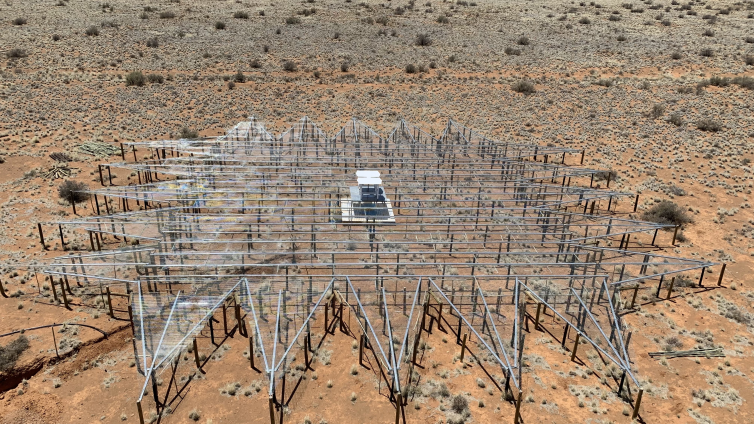
\includegraphics[width=0.8\textwidth]{antenna.png}
	\end{figure}

	\begin{center}
		\begin{tikzpicture}
			\node[draw, rounded corners, inner sep=10pt] (box) {%
				\begin{minipage}{0.9\textwidth} % Width of the box
					\begin{columns}[c] % Align columns centrally inside the box
						\begin{column}{0.33\textwidth}
							\centering
							{\small We measure \textit{sky averaged} signal.}
						\end{column}
						\begin{column}{0.33\textwidth}
							\centering
							{\small Antenna  LNA impedance mismatch}
						\end{column}
						\begin{column}{0.33\textwidth}
							\centering
							{\small Very faint signal.}
						\end{column}
					\end{columns}
				\end{minipage}
			};
		\end{tikzpicture}
	\end{center}

\end{frame}

\begin{frame}{\small{How to calibrate (in a bit more detail...)?}}
	\vspace{-0.5cm}
	\begin{flushleft}
		\textbf{Objective:} Map input temperature to output power.
		\vspace{0.2cm}

		\textbf{Key Factors:}
		\begin{itemize}
			\item LNA introduces time-dependent gain, $g(t)$.
			\item Impedance mismatch adds noise ($T_{\text{rec}}$) to the system.
		\end{itemize}

		\vspace{0.2cm}
		\textbf{Output Power Equation:}
	\end{flushleft}

	% Apply \tiny to the entire equation by wrapping it in a group
	{
	\begin{equation}
		P_{\text{out}}^{\text{src}} = g M \left( T_{\text{in}}^{\text{src}} + T_{\text{rec}} \right) \tag{1}
	\end{equation}
	}

	\vfill % Pushes the following content to the bottom

	\begin{footnotesize}
		\textit{Note: All parameters above are frequency-dependent, but the notation has been simplified here and thereafter for convenience.}
	\end{footnotesize}

\end{frame}

\begin{frame}{\small{Dealing with reflections...}}

	% Output Power Equation without title, maintaining the same equation number (1)
	{\tiny
		\begin{equation}
			P_{\text{out}}^{\text{src}} = \textcolor{red}{g} M \left( T_{\text{in}}^{\text{src}} + \textcolor{red}{T_{\text{rec}}} \right) \tag{1}
		\end{equation}
	}

	\vspace{0.3cm}
	\hrule  % Horizontal line for separation
	\vspace{0.3cm}

	% Noise Parameter Equation with smaller, uniform title
	\textbf{\small{Noise Parameter Equation:}}
	{\tiny
		\begin{equation}
			P_{\text{out}}^{\text{src}} = \textcolor{red}{g} M \left( T_{\text{in}}^{\text{src}} + \textcolor{red}{T_{\text{min}}} + T_0 \frac{4\textcolor{red}{R_N}}{Z_0} \frac{|\Gamma_{\text{src}} - \textcolor{red}{\Gamma_{\text{opt}}}|^2}{(1 - |\Gamma_{\text{src}}|^2)(1 + |\Gamma_{\text{opt}}|^2)} \right) \tag{2}
		\end{equation}
	}

	\vspace{0.3cm}
	\hrule  % Horizontal line for separation
	\vspace{0.3cm}

	% Noise Wave Equation with smaller, uniform title
	\textbf{\small{Noise Wave Equation:}}

	{\tiny
		\begin{multline}\label{}
			P_{\text{out}}^{\text{src}} = \textcolor{red}{g} \left[ \textcolor{red}{T_0} + \textcolor{red}{T_{\text{unc}}} |\Gamma_{\text{s}}|^2 \left|\frac{ \sqrt{1 - |\Gamma_{\text{rec}}|^2}}{1 - \Gamma_{\text{s}}\Gamma_{\text{rec}}} \right|^2 \right. \\
				\left. + T_{\text{s}}(1 - |\Gamma_{\text{s}}|^2) \left|\frac{ \sqrt{1 - |\Gamma_{\text{rec}}|^2}}{1 - \Gamma_{\text{s}}\Gamma_{\text{rec}}} \right|^2 + \textcolor{red}{T_{\text{cos}}} \Re \left( \Gamma_{\text{s}} \frac{\sqrt{1 - |\Gamma_{\text{rec}}|^2}}{1 - \Gamma_{\text{s}} \Gamma_{\text{rec}}} \right) \right. \\
				\left. + \textcolor{red}{T_{\text{sin}}} \Im \left( \Gamma_{\text{s}} \frac{\sqrt{1 - |\Gamma_{\text{rec}}|^2}}{1 - \Gamma_{\text{s}} \Gamma_{\text{rec}}} \right) \right] \tag{3}
		\end{multline}
	}

\end{frame}

\begin{frame}{\small{Calibration Equation}}

	\vspace{0.2cm} % Adds a small vertical space at the top

	\textbf{Typically, substitute in the noise wave parameter equation here (gains cancel)}

	\vspace{0.2cm} % Adds space between text and first equation

	% Calibration Equation with \tiny font and manual tag (4)
	{\tiny
		\begin{equation}
			T_{\text{cal}}^* = T_{\text{NS}} \frac{P_{\text{cal}} - P_L}{P_{\text{NS}} - P_L} + T_L \tag{4}
		\end{equation}
	}

	\vspace{0.3cm} % Adds space between equation and next text

	\textbf{Make some matching assumptions and re arrange:}

	\vspace{0.2cm} % Adds space between text and second equation

	% Multline Equation with \tiny font and manual tag (5)
	{\tiny
		\begin{multline}
			T_\mathrm{s} = \textcolor{red}{T_\mathrm{NS}}\left(\frac{P_\mathrm{s} - P_\mathrm{L}}{P_\mathrm{NS} - P_\mathrm{L}}\right)\frac{\left|1 - \Gamma_\mathrm{s}\Gamma_\mathrm{rec}\right|^2}{1 - |\Gamma_\mathrm{s}|^2} + \textcolor{red}{T_\mathrm{L}}\frac{\left|1 - \Gamma_\mathrm{s}\Gamma_\mathrm{rec}\right|^2}{1 - |\Gamma_\mathrm{s}|^2} - \textcolor{red}{T_\mathrm{unc}} \frac{|\Gamma_\mathrm{s}|^2}{1 - |\Gamma_\mathrm{s}|^2} +  \\
			-\textcolor{red}{T_\mathrm{cos}} \frac{\Re \left( \frac{\Gamma_\mathrm{s}}{1 - \Gamma_\mathrm{s}\Gamma_\mathrm{rec}} \right)\left|1 - \Gamma_\mathrm{s}\Gamma_\mathrm{rec}\right|^2}{(1 - |\Gamma_\mathrm{s}|^2) \sqrt{1 - |\Gamma_\mathrm{rec}|^2}}  -\textcolor{red}{T_\mathrm{sin}} \frac{\Im \left( \frac{\Gamma_\mathrm{s}}{1 - \Gamma_\mathrm{s}\Gamma_\mathrm{rec}} \right)\left|1 - \Gamma_\mathrm{s}\Gamma_\mathrm{rec}\right|^2}{(1 - |\Gamma_\mathrm{s}|^2) \sqrt{1 - |\Gamma_\mathrm{rec}|^2}} \tag{5}
		\end{multline}
	}

	\textit{Note: We end up with 5 parameters that need to be estimated to calibrate the system.}

	\vfill % Pushes the note to the bottom
\end{frame}

\begin{frame}{Calculating the error}

	% Adding a block
	\begin{block}{By partial derivatives}
		To find the error in \( T_s \), we propagate the errors in \( \Gamma_s \), \( \Gamma_{rec} \), \( P_L \), \( P_{NS} \), and \( P_s \):
		%
		\begin{multline}
			(\Delta T_s)^2 = \left(\frac{\partial T_s}{\partial \Gamma_s} \Delta \Gamma_s\right)^2 + \left(\frac{\partial T_s}{\partial \Gamma_{rec}} \Delta \Gamma_{rec}\right)^2 \\ + \left(\frac{\partial T_s}{\partial P_L} \Delta P_L\right)^2 + \left(\frac{\partial T_s}{\partial P_{NS}} \Delta P_{NS}\right)^2 + \left(\frac{\partial T_s}{\partial P_s} \Delta P_s\right)^2.\label{eq:errordicke} \tag{6}
		\end{multline}
		%
	\end{block}

\end{frame}



\begin{frame}{Calculating the error}

	% Adding a block
	\begin{block}{By partial derivatives}
		To find the error in \( T_s \), we propagate the errors in \( \Gamma_s \), \( \Gamma_{rec} \), \( P_L \), \( P_{NS} \), and \( P_s \):
		%
		\begin{multline}\small
			(\Delta T_s)^2 = \left(\frac{\partial T_s}{\partial \Gamma_s} \Delta \Gamma_s\right)^2 + \left(\frac{\partial T_s}{\partial \Gamma_{rec}} \Delta \Gamma_{rec}\right)^2 \\ + \left(\frac{\partial T_s}{\partial P_L} \Delta P_L\right)^2 + \left(\frac{\partial T_s}{\partial P_{NS}} \Delta P_{NS}\right)^2 + \left(\frac{\partial T_s}{\partial P_s} \Delta P_s\right)^2.\label{eq:errordicke} \tag{6}
		\end{multline}
		%
	\end{block}

	\hrule


	\begin{columns}[c] % Align columns centrally inside the box
		\begin{column}{0.5\textwidth}
			\centering
			{\tiny
				\begin{align}		\frac{\partial T_s}{\partial P_L}    & = T_\mathrm{NS} \frac{\left|1 - \Gamma_\mathrm{s} \Gamma_\mathrm{rec}\right|^2}{1 - |\Gamma_\mathrm{s}|^2} \cdot \frac{P_\mathrm{s} - P_\mathrm{NS}}{(P_\mathrm{NS} - P_\mathrm{L})^2}. \\
               \frac{\partial T_s}{\partial P_{NS}} & = -T_\mathrm{NS} \frac{\left|1 - \Gamma_\mathrm{s} \Gamma_\mathrm{rec}\right|^2}{1 - |\Gamma_\mathrm{s}|^2} \cdot \frac{P_\mathrm{s} - P_\mathrm{L}}{(P_\mathrm{NS} - P_\mathrm{L})^2}. \\
               \frac{\partial T_s}{\partial P_s}    & = T_\mathrm{NS} \left(\frac{1}{P_\mathrm{NS}-P_\mathrm{L}}\right) \frac{\left|1-\Gamma_\mathrm{s}\Gamma_\mathrm{rec}\right|^2}{ 1-|\Gamma_\mathrm{s}|^2}.
				\end{align}
			}
		\end{column}
		\begin{column}{0.5\textwidth}
			\centering
			{\small Gamma error eqn's here}
		\end{column}
	\end{columns}
\end{frame}

\begin{frame}{Calculating the error}

	% Adding a block
	\begin{block}{Using $T_{\text{NS}} \frac{P_{\text{cal}} - P_L}{P_{\text{NS}} - P_L} + T_L$ \tag{4}}
		%
		\begin{align}
			(\Delta T_s)^2 & = \left(\frac{\partial T_s}{\partial P_s} \Delta P_s\right)^2 + \left(\frac{\partial T_s}{\partial P_L} \Delta P_L\right)^2 + \left(\frac{\partial T_s}{\partial P_{NS}} \Delta P_{NS}\right)^2 \\ &+ \left(\frac{\partial T_s}{\partial \Gamma_s} \Delta \Gamma_s\right)^2 + \left(\frac{\partial T_s}{\partial \Gamma_{rec}} \Delta \Gamma_{rec}\right)^2. \label{eq:errordicke} \tag{6}
		\end{align}
		%
	\end{block}


	\begin{block}{Using noise wave parameters \textit{only}}
		%
		\begin{align}
			(\Delta T_\mathrm{s})^2 & = \left(\frac{\partial T_\mathrm{s}}{\partial P_\mathrm{s}} \Delta P_\mathrm{s}\right)^2 \\ &+ \left(\frac{\partial T_\mathrm{s}}{\partial \Gamma_\mathrm{s}} \Delta \Gamma_\mathrm{s}\right)^2 + \left(\frac{\partial T_\mathrm{s}}{\partial \Gamma_\mathrm{rec}} \Delta \Gamma_\mathrm{rec}\right)^2.\label{nodicke}
		\end{align}
		%
	\end{block}

\end{frame}

\begin{frame}
	\begin{figure}[h]
		\centering
		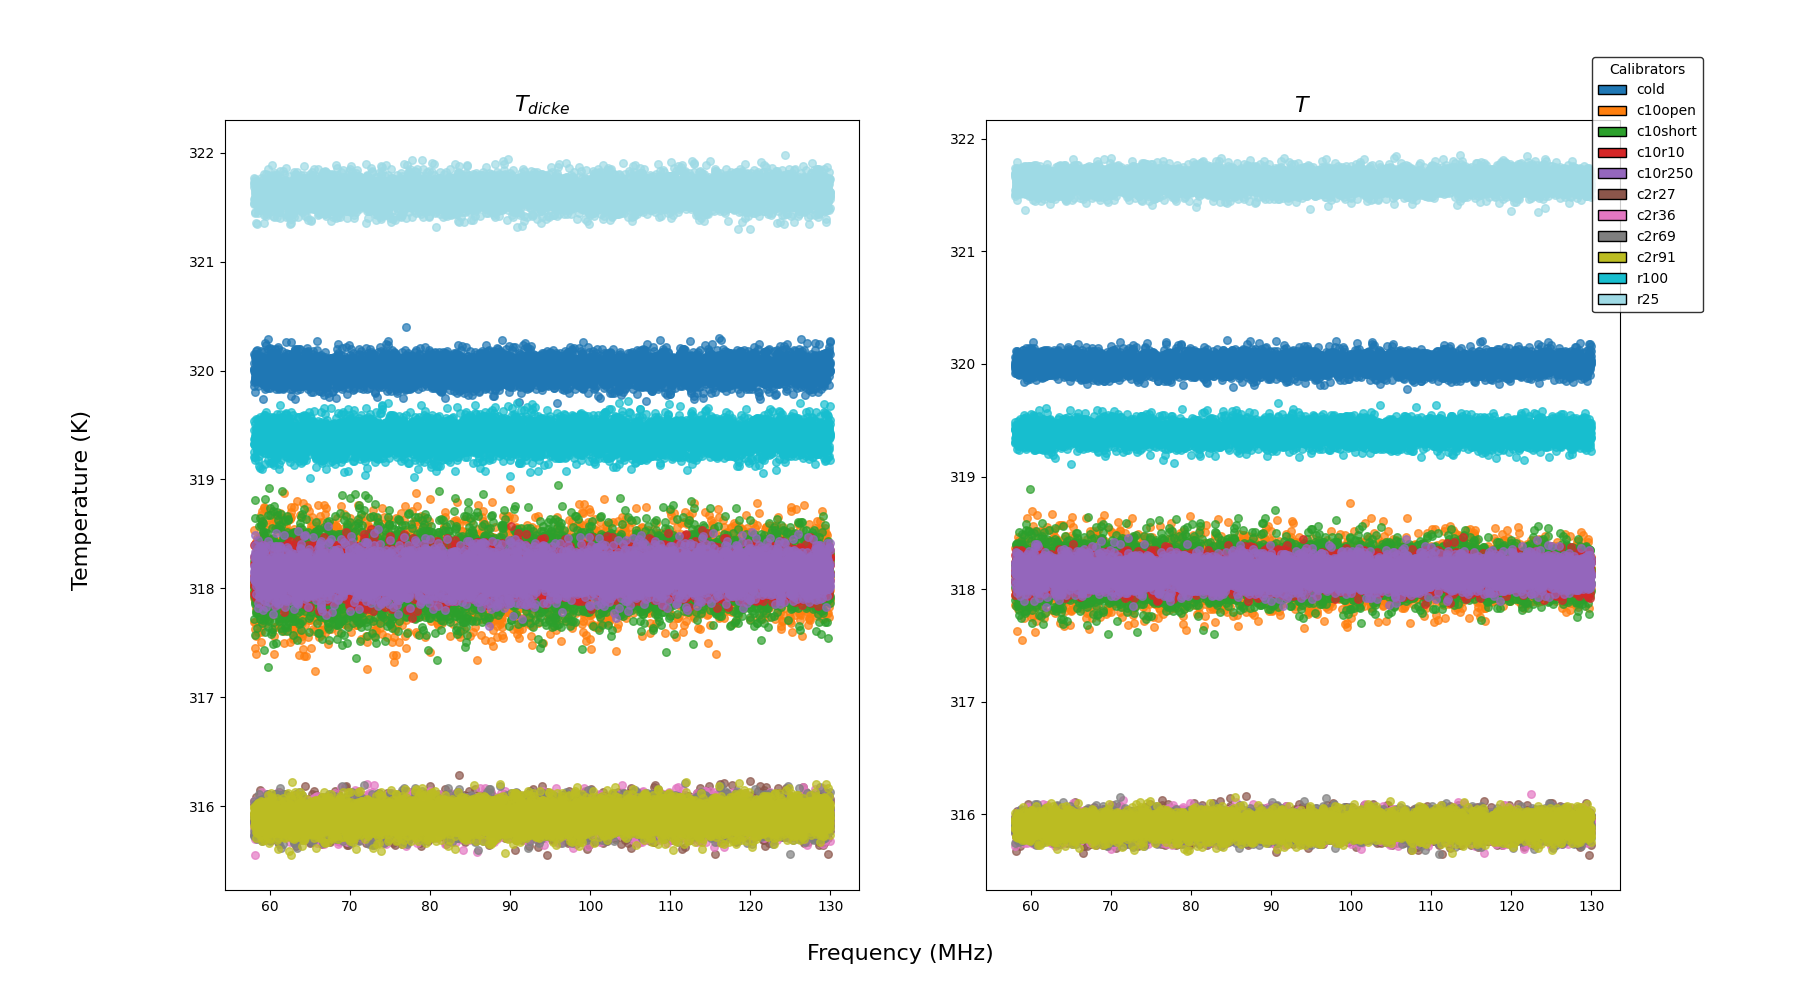
\includegraphics[width=1\textwidth]{main_scatter_plots.png}
		\caption{Caption for the image.}
		\label{fig:image1}
	\end{figure}
\end{frame}


\begin{frame}
	\begin{figure}[h]
		\centering
		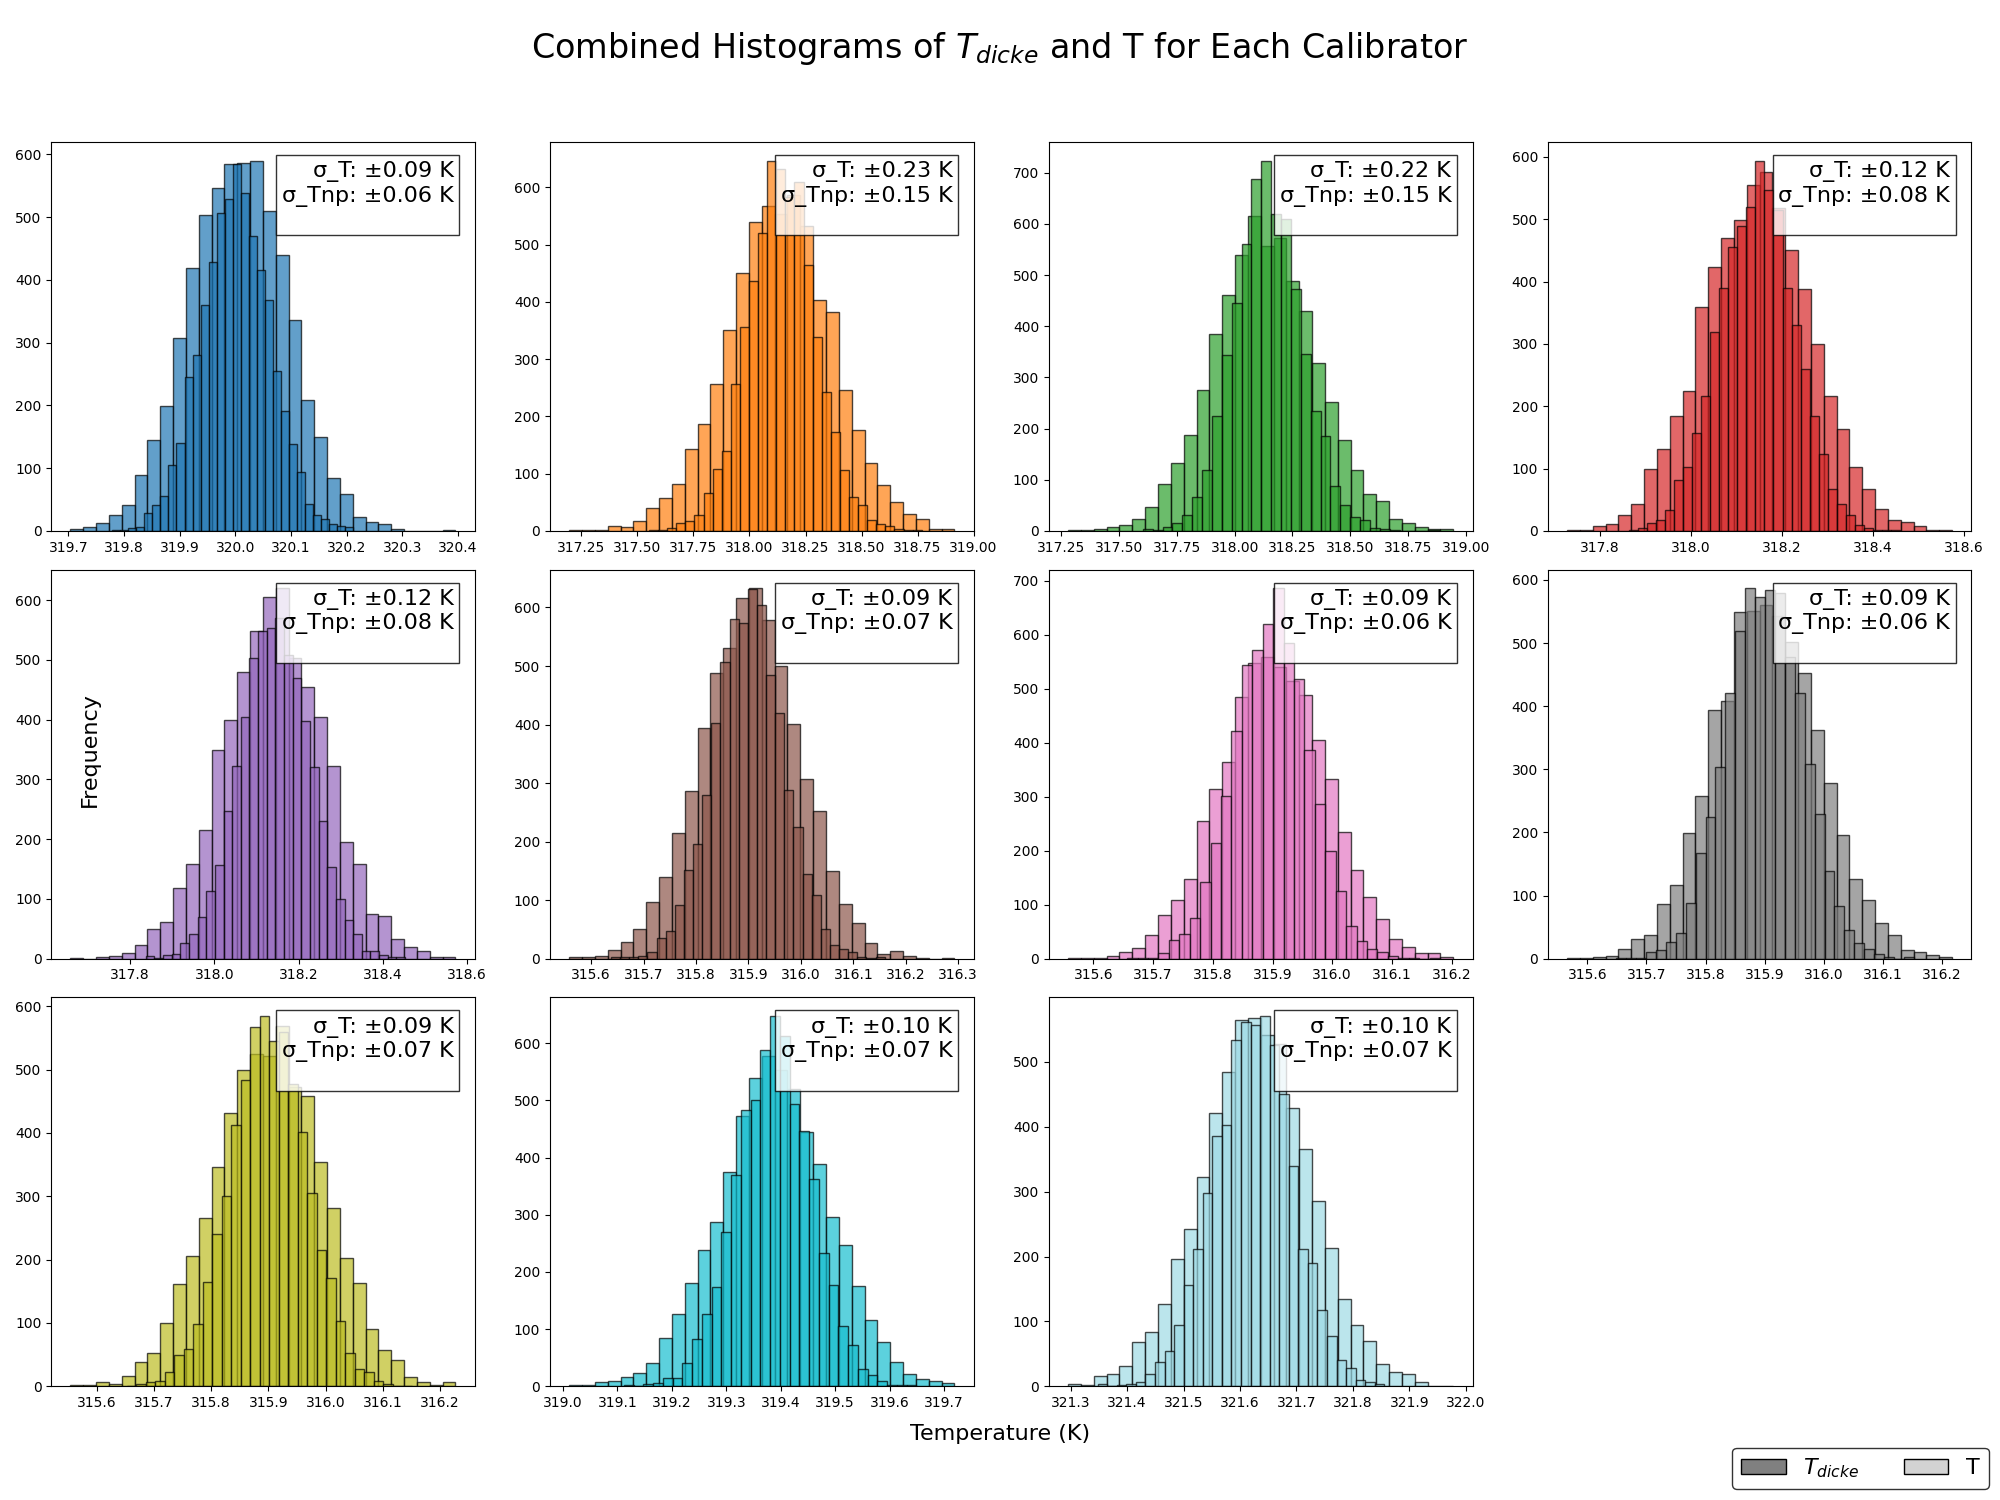
\includegraphics[width=1\textwidth]{combined_histograms.png}
		\caption{Caption for the image.}
		\label{fig:image1}
	\end{figure}
\end{frame}

\begin{frame}{Why not fit noise (wave) parameters directly?}

	% Noise Parameter Equation with smaller, uniform title
	\textbf{\small{Noise Parameter Equation:}}
	{\tiny
		\begin{equation}
			P_{\text{out}}^{\text{src}} = \textcolor{red}{g} M \left( T_{\text{in}}^{\text{src}} + \textcolor{red}{T_{\text{min}}} + T_0 \frac{4\textcolor{red}{R_N}}{Z_0} \frac{|\Gamma_{\text{src}} - \textcolor{red}{\Gamma_{\text{opt}}}|^2}{(1 - |\Gamma_{\text{src}}|^2)(1 + |\Gamma_{\text{opt}}|^2)} \right) \tag{2}
		\end{equation}
	}

	\vspace{0.3cm}
	\hrule  % Horizontal line for separation
	\vspace{0.3cm}

	% Noise Wave Equation with smaller, uniform title
	\textbf{\small{Noise Wave Equation:}}

	{\tiny
		\begin{multline}\label{}
			P_{\text{out}}^{\text{src}} = \textcolor{red}{g} \left[ \textcolor{red}{T_0} + \textcolor{red}{T_{\text{unc}}} |\Gamma_{\text{s}}|^2 \left|\frac{ \sqrt{1 - |\Gamma_{\text{rec}}|^2}}{1 - \Gamma_{\text{s}}\Gamma_{\text{rec}}} \right|^2 \right. \\
				\left. + T_{\text{s}}(1 - |\Gamma_{\text{s}}|^2) \left|\frac{ \sqrt{1 - |\Gamma_{\text{rec}}|^2}}{1 - \Gamma_{\text{s}}\Gamma_{\text{rec}}} \right|^2 + \textcolor{red}{T_{\text{cos}}} \Re \left( \Gamma_{\text{s}} \frac{\sqrt{1 - |\Gamma_{\text{rec}}|^2}}{1 - \Gamma_{\text{s}} \Gamma_{\text{rec}}} \right) \right. \\
				\left. + \textcolor{red}{T_{\text{sin}}} \Im \left( \Gamma_{\text{s}} \frac{\sqrt{1 - |\Gamma_{\text{rec}}|^2}}{1 - \Gamma_{\text{s}} \Gamma_{\text{rec}}} \right) \right] \tag{3}
			  \end{multline}
			}

			\textit{We still end up with 5 unknowns, as before.}

\end{frame}

\begin{frame}{\small{Machine learning for radiometer calibration in global 21cm cosmology}}
	\begin{figure}
		\centering
		\includesvg[width=1.05\textwidth]{instrument.svg}
	\end{figure}
	\vfill
\end{frame}

\begin{frame}{\small{Machine learning for radiometer calibration in global 21cm cosmology}}
	\begin{figure}
		\centering
		\includesvg[width=0.9\textwidth]{nn.svg}
	\end{figure}
	\vfill
\end{frame}

\begin{frame}{\small{Machine learning for radiometer calibration in global 21cm cosmology}}
	\begin{figure}
		\centering
		\includesvg[width=1\textwidth]{results.svg}
	\end{figure}

	\begin{figure}
		\centering
		\includesvg[width=0.3\textwidth]{nn.svg}
	\end{figure}
	\vfill
\end{frame}

\begin{frame}{\small{Thank you!}}
	\begin{figure}
		\centering
		
\includegraphics[width=0.55\textwidth]{qr.png}
	\end{figure}
\end{frame}

\end{document}
